\section*{Synthesizing Measures of State Preference}

The approach that we introduce here to measure state preferences starts by assuming that both UN voting and alliance relationships are sources of information on how states relate to one another on the international stage. By accounting for the multiple layers upon which states interact with one another we can synthesize a better measure of state preferences than if we relied on any one measure alone.\footnote{The idea of using multiple metrics to get a better handle on preferences is not new, in fact, Signorino and Ritter suggested it in introducing S-scores, which were designed to allow for aggregation of similarity on multiple dimensions (such as alliances and UN voting).} The downside of this extant approach, however, is that it does not account for structural patterns that we often see in relational data. 

Relational data is composed of observations between pairs of actors, or dyads. For both alliance relationships and UN voting, we are able to observe how the actors in the international system interact with one another across time. This system of interactions taken in its totality defines a network, and within these types of structures a bevy of research has shown that we need methods that go beyond assuming that interactions are taking place between just two actors in a vacuum \citep{wasserman:faust:1994,snijders:nowicki:1997,minhas:etal:2019}. As such we reformulate the problem of determining state preferences in terms of a network analysis. The goal of our approach is summarized in Figure~\ref{fig:tensViz}. In the top row, we represent UN voting and alliance patterns at time $t$ as a pair of adjacency matrices that form an evolving multiplex network.\footnote{The approach that we describe here can be generalized to a multiplex with more than two dimensions.} Our goal is to extract a lower dimensional representation of this system, such that the output is a series of $n \times n$ matrices, where $n$ represents the number of actors and in which the cross-sections denote our estimates of the preference similarities between countries.

% needs to be modified
% prolly dont need this simplistic representation for a networks audience
\begin{figure}[ht]
	\centering
	% \resizebox{.8\textwidth}{!}{\input{dimRedStrat.tex}}
	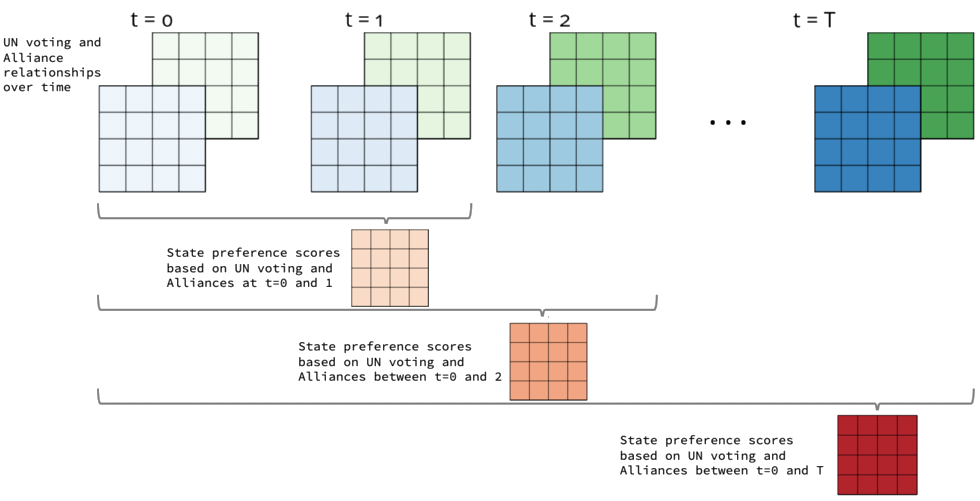
\includegraphics[width=1\textwidth]{tensor_viz.png}
	\caption{The green and blue colors represent different relational measures and darker shading indicates later time periods. Our goal is to reduce the patterns found across those layers of relationships into a single measure.}
	\label{fig:tensViz}
\end{figure}

We generate these estimates through a multilinear tensor regression model that combines information across networks and time to measure how dependent the actions of a particular state is on another. We will show that by combining different measures of state preferences, and better accounting for network dependencies through our approach, we are able to generate a measure for preference that maintains the insights of both UN voting scores and S-scores and which can yield new insights, in particular when it comes to predicting and explaining interstate conflict.

\subsection*{Multilayer Tensor Decomposition}

In essence, our goal here is to measure an unobservable concept. This is a problem that is very familiar in political science and a number of techniques based on measurement models have been developed to study political ideology \citep{martin:quinn:2002,konig:etal:2013}, human rights abuses \citep{fariss:2014}, and judicial independence \citep{linzer:staton:2015}. Obviously, the ideal points measure developed by \citet{bailey:etal:2015} also follows in this growing practice of extracting unobserved information via a spatial weighting scheme. Here we employ this general framework to develop a measurement of how a state relates to other states in a network context. Substantively, this goal is no different than how others have sought to find simpler representations of legislators and bills \citep{poole:rosenthal:1985,clinton:etal:2004}.

% However, in the network case there are specific types of patterns that often occur and that should be captured when reducing the dimensionality of a network. One such pattern is stochastic equivalence. Stochastic equivalence refers to the idea that there are communities of nodes in a network, and actors within a community act similarly towards those in other communities. Thus the community membership of an actor provides us with information on how that actor will act towards others in the network. Put more concretely, a pair of actors $ij$ are stochastically equivalent if the probability of $i$ relating to, and being related to, by every other actor is the same as the probability for $j$ \citep{anderson:etal:1992}. This concept simply speaks to the assertion that we can learn something about how an actor will interact with an entire network based on, for example, the existing set of alliances that they are enmeshed in.

% An additional dependence pattern that often manifests in networks is homophily -- the tendency of actors to form links they share some latent attribute. In many cases, homophily will lead to greater levels of transitivity in a network because, if $i$ and $j$ share an attribute and thus are more likely to be linked, and $j$ and $k$ share the same attribute and are linked, then we should expect to see a link between $i$ and $k$. In the context of clustering in alliance relationships, we are likely to find that states like the United States, United Kingdom, and Germany may cluster together because they share some latent state level attribute. We would ignore salient information if we did not use, for example, the United Kingdom's behavior towards third parties, when trying to understand the United States' preference similarity with those parties. Doing so is likely to paint an incomplete picture of the preferences that states share with one another.

% \section*{Modeling Approach}

% In our model, we go a step further by estimating the relationship between trade and conflict in a multilinear tensor regression. Our estimation approach here utilizes the framework established in Hoff (2015) and Minhas et al. (2016). We review the approach briefly here. 

% \subsection*{Tensor Model}

We represent relational data that is longitudinal be represented as a series of matrices $\{\bl Y_t : t = 1, \ldots n\}$, with each $\bl Y_t$ representing the actions or flows between the pairs of actors, in our case countries, at a given month $t$. A cross-sectional entry such as $y_{i,j,v,t}$ from $\bl Y_t$ denotes an interaction that occurred between actors $i$ and $j$ at time $t$ across variable $v$. These series of matrices can be assembled in a tensor, $\bl Y$, which we use to represents actors interacting over time across multiple measures. Specifically, $\bl Y$ will have dimensions $m \times m \times v \times n$, where $m$ corresponds to the number of countries, $v$ to the number of variables (i.e., relational measures), and $n$ to the number of time periods. Figure~\ref{fig:tensViz} provides an example of this for the simple case of four countries, three time points, and two relational measures. 

% $\bl Y$ 
Now we can also rewrite the information contained in this set of matrices as a vector, where $(\mathbf y_t)$ represents a time series of vectors representing the dyadic interactions across multiple variables for $m$ countries through the period $t = 1, \ldots, n$. Transforming the data in this way enables us to think of what we are modeling in an explicitly time series context, where the evolution of multiple series is a function of their past behavior. Modeling such processes can often be accomplished using a vector autoregression (VAR) framework.The benefit of this approach is that it models a set of time series as resulting from a dynamic and endogenous process, rather than imposing a priori assumptions of exogeneity between the various explanatory variables, and we can posit the autoregressive relation as:

\begin{eqnarray}
	\bl y_t &=& { \Theta \bl y_{t-1} +\bl e_t}\\
	E[\bl e_t] &=& 0 \\
	E[\bl e_t \bl e^T_s] &=& \begin{cases}   \Sigma &\mbox{if } t=s, \\ 0 &\mbox{otherwise}\end{cases}
\end{eqnarray}

\noindent where $\bl y_t$ has been demeaned to eliminate intercepts such that $\sum_t y_{i,j,t}/n \equiv 0$. This is easy to estimate, but has extreme data requirements since $ \Theta$ has $m^4$ entries. One basic solution to this is to use a bilinear model such that the regression matrix is given by $ \Theta = \bl B \otimes \bl A$, where $\otimes$ is the Kronecker product. As a result of this specification we obtain a basic specification that somewhat mimics alternatives approaches to modeling cross-sectional networks such as the latent factor model (see Minhas et al. (2019)): $\bl Y_t = \bl A \bl Y_{t-1}\bl B^T$.The key difference here, however, is that in latent factor models we are projecting the relations between actors onto lower a dimensional space, where similarity in orientation indicates that actors are more likely to have similar dependence patterns. In the context of this model, $\bl A$ and $\bl B$ are $m \times m$ matrices of regressions coefficients, where each cross-sectional entry measures the level of dependence between the sending relationships of a particular actor and the $B$ the receiving relationships. 

$a_{i,i'}$ capture how previous actions of $i'$ affect $i$ and $b_{j,j'}$ shows how actions that target $j$ are influenced by prior actions toward $j'$. If $a_{i,i'}$ is positive, this gives us a measure of how likely $i$ is to send an event to a third party $k$ givent that $i'$ has already sent an event to $k$. More concretely, if we imagine that the event is verbal cooperation, then a positive $a_{i,i'}$ would indicate that $i$ and $i'$ are more likely to send cooperative events to the same third country. If $b_{j,j'}$ is positive on the other hand, this gives us a measure of how likely $j$ is to receive an event from a third party $k$ given that $j'$ has already received an event from $k$. Another way would be to think of this is $b_{j,j'}>0$ gives us a warning that if $j'$ has been attacked by $k$, then $k$'s $j$ should expect to be attacked soon as well. 

Given these parameters, the model for a single country-country-variable observation is shown in equation~\ref{eqn:mltrObs}, where $i$ represents a sender country, $j$ a target, $k$ a particular relational variable, and $t$ a time point: 

\begin{equation}  
	y_{ijvt} = \sum_i' \sum_j' \sum_k' a_{1ii'} b_{2jj'} b_{3kk'} x_{i'j'k't}
	\label{eqn:mltrObs}
\end{equation}

The regression problem can also be written somewhat more simply in tensor form, where it is clearer that we are essentially regressing the relational tensor $\bl Y_t$ from time $t$ on the tensor $\bl X_t =\bl Y_{t-1}$ from time $t-1$:

\begin{equation}  
	\bl Y = \bl X \boldsymbol{\times} \{ \bl A, \bl B, \bl \beta \} + \bl E ,  
	\label{eqn:mltr}
\end{equation}

\noindent where ``$\boldsymbol{\times}$'' is a multilinear operator known as the ``Tucker product''.\footnote{The Tucker product is a multilinear operator that is used for higher-order singular value decomposition (SVD), the same way that matrix multiplication is used for matrix SVD (Kolda \& Bader 2009). To illustrate how the Tucker product is calculated, say that we want to get the following expression: $\bl Y = \bl X \boldsymbol{\times} \{ \bl A, \bl B, \bl B_{3}\},$ where $\bl Y$ has dimensions $n_{1} \times n_{2} \times n_{3}$ and $\bl X$ has dimensions $m_{1} \times m_{2} \times m_{3}$. The first step involves reshaping $\bl X$ so that it is a matrix with  dimensions $m_{1} \times (m_{2} \times m_{3})$, then we multiply on the left by $\bl B$, next we reshape the result to an $n_{1} \times m_{2} \times m_{3}$ matrix. This procedure would be applied iteratively among the remaining dimensions. Further details on this operator can be found in: Kolda (2006).} Here $\bl Y$ and $\bl X$ are $m \times m \times v \times n$ tensors and each entry for $\bl X$ is lagged by one period. 

Thus $\bl A$ and $\bl B$ represent how previous actions along any of the $v$ parameters affects future interactions. For example, the $i j$ coefficient in $\bl A$ measures the effect of an interaction from actor $j$ to actor $k$ along any of the $v$ parameters on the likelihood of an interaction from $i$ to $k$, in any of the parameters, in the next time period.\footnote{For example, for each county $i$, the coefficient $b_{1iUSA}$ describes how predictive the actions of the USA are of the future actions of country $i$. Heterogeneity of these coefficients across countries $i$ describes heterogeneity of the nodes in terms of their dependence on the actions of USA.}

The key output from the LFM for our purpose here is $U \Lambda U^{\top}$. Actor positions in the latent factor space are characterized by the concepts of homophily and stochastic equivalence  discussed above. Interpretation of this space needs to be done with care. Distances between actors cannot be interpreted using Euclidean metrics, as actor's latent positions are actually embedded within a k-dimensional hypersphere. This means that an actor's vector direction within the k-dimensional hypersphere indicates which latent preferences an actor $i$ has and does not have. Comparing the similarity of preferences between two states, $\{i,j\}$, can be accomplished by comparing the direction to which their respective factor vectors point. A commonly used metric for this sort of problem in the recommender system literature from computer science is the cosine of the angle formed by the latent vectors of both actors.\footnote{For a review of this literature see \citep{amatriain:etal:2015}.} We refer to this distance metric as latent angle distance.\footnote{This measure is defined as: $\text{Latent angle distance}_{ij} = \frac{u_{i} \cdot u_{j}}{||u_{i}|| \cdot ||u_{j}||}$.} Thus, if the estimated latent vectors of two states are in the same direction, they are apt to have both alliances and UN co-voting to similar partners. The way we measure this similarity in dimension is by looking at the absolute distance of the angles created by each states position and the center of the latent space. 

As an example of how our tensor dependence measure is effected by changes in alliance relations or UN voting similarity consider the United States and Israel, in 1981. With the signing of the ``Joint Memorandum of Understanding," the two states went from having no alliance relationship to having one, the states were voting together at the UN 80\% of the time (up 3\% from 1980, below the median yearly change for this dyad). These factors, coupled with changes in the third order effects for the dyad, led the tensor dependency to increase from about 2.72 to about 3.08. 

\textcolor{red}{Can you put in the explicit math that leads to this SM?} 

Of course, another pair of countries might sign an alliance (or withdraw from an alliance) and have a markedly different effect on this measure of tensor dependency. For example, in 1977, the United Kingdom and the United States went from being in 5 alliances together to being in 4, and this led to a drop in their tensor dependency from 3.13 to 2.28, despite a decrease in their UN voting similarity of less than 1\%. This is because the alliance that ended in 1977 was the Southeast Asian Treaty Organization, which had 4 other members, and so the third order effects were concomittantly more severe. To capture the aggregate effects of dyadic variables on our measure of tensor dependency, we estimated a simple linear model, depicted in table \ref{tensor:ols}, and these dyadic factors account for about 78\% of the variance, with the rest coming from third order factors. 

\begin{table}[ht]
	\centering
	\begin{tabular}{lcccc}
		\hline
		& Estimate & Std. Error & t value & Pr($>|t|$) \\ 
		\hline
		(Intercept) & 0.0773 & 0.001 & 74.26 & 0.000 \\ 
		Tensor Dependence$_{t-1}$ & 0.888 & 0.0004 & 2094.81 & 0.000 \\ 
		Change in Alliance Relationship & 0.131 & 0.009 & 15.30 & 0.000 \\ 
		Change in UN Voting Similarity & 4.401 & 0.014 & 313.14 & 0.000 \\ 
		\hline
	\end{tabular}
	\label{tensor:ols}
	\caption{Regression of tensor dependence on dyadic components.}
\end{table}


% We account for higher order dependence patterns using a latent factor model (LFM) that allows us to capture both concepts discussed above: the tendency of actors to assort themselves into groups and to form transitive links \citep{hoff:2005,hoff:etal:2013,minhas:etal:2018}. Using the LFM ensures that similarity in preferences are likely to be transitive, for example, if the United States has similar preferences to the United Kingdom, and the United Kingdom to France, the United States' preferences should be relatively close to France's. Further the most useful feature of the LFM for our purpose is that it places actors it summarizes the interdependencies between actors in a relational k-dimensional latent vector space. Thus, the model we use does a better job of capturing the interdependencies in both alliance and voting data than we would expect from the literature. From this space we can not only approximate how pairs of countries relate to one another, but also estimate how an actor may relate to a cluster of other actors or the international system as a whole. Actors that have vectors pointing in similar directions are more likely to have similar state preferences based on their alliances and UN voting records. The angle between the vectors for actors $i$ and $j$ provides an estimate of how similar the state preferences of $i$ are to $j$. 

% To generate this measure, scholars would begin by constructing $T$ different $n \times n \times p$ arrays, where $T$ represents the number of periods, $n$ represents the number of actors,\footnote{The number of actors can vary by period.} and $p$ the number of observed variables used to synthesize a measure of state preference. For the application that we focus on in the next section, both alliance relationships and UN voting scores are undirected measures, meaning that $y_{ij} = y_{ji} \; \forall \; p \text{ and } t$.\footnote{The approach we describe can also be generalized to the case where $y_{ij} \neq y_{ji}$.} In order to obtain a lower-dimension relational measure of state preferences, we use the LFM separately for each time point: 

% \begin{align*}
% 	Y &= f(\theta)\\
% 	\theta &= \beta^{\top} X + Z \\
% 	Z &= M + E  \\
% 	M &= U \Lambda U^{\top}\text{, where } \\
% 	&\qquad u_{i} \in \rm I\!R^{k} \text{ and } \\ 
% 	&\qquad \Lambda \text{ is a } k \times k \text{ diagonal matrix}
% \end{align*}

% \noindent where $f(.)$ is a general link function corresponding to the distribution of $Y$ and $\beta^{\top}\mathbf{X}$ is the standard regression term for dyadic and nodal fixed effects. In this application, for the sake of parsimony we abstain from using fixed effects. However, if one was interested in estimating a measure of preference that parsed out the effect of geographic distance between $i$ and $j$, for example, than this could be accomplished within the context of this framework by simply including that as a covariate in the $X$ design array. $Z$ represents any additional patterns in data unrelated to the specified dyadic and nodal fixed effects. To incorporate multiple measures of similarity into a single ideal point estimation, we treat each different slice of data as arising from a common distribution. In this way, each additional observed relationship between actors that we add serves to provide additional information to the model that can be used to estimate a latent measure of state preference. 

% The key part of this model lies in the decomposition of $Z$. Specifically, we can write $Z = M + E$ such that the matrix $E$ represents noise, and $M$ is systematic effects. By matrix theory, we can factorize $M$ into the product of two simpler matrices: $M = U \Lambda U^{\top}$, where $u_{i} \in \rm I\!R^{k}$ is a latent vector associated to node $i$ and $\Lambda$ is a $k \times k$ diagonal matrix. Thus under this framework a vector of latent characteristics are estimated for each actor, $u_{i} = \{u_{i,1}, \ldots, u_{i,k}\}$. Similarity in the latent factors between two actors, $u_{i} \approx u_{j}$, corresponds to how stochastically equivalent they are and the diagonal entries in $\Lambda$, $\lambda_{k} > 0 \text{ or } \lambda_{k} < 0$, determine the level of homophily (or antihomophily) in the network \citep{minhas:etal:2018}. Within this framework, the LFM can represent either positive or negative homophily in varying degrees and stochastially equivalent actors may or may not share strong relationships with others in their ``community''.\footnote{This model does assume, once we condition on the latent factor $U \Lambda U^{\top}$, that relations are independent, but this factor has been found to capture the different dependencies that have been theorized to be present in both alliance and voting behavior.}

% Inference of the latent vectors for each actor takes place within the context of a MCMC procedure that enables us to construct approximate samples from the posterior distributions of the latent variables. For the latent factor model, a diffuse normal prior is placed on $\Lambda$ and the prior distribution on $U$ is taken to be a uniform distribution. The MCMC proceeds by sampling the parameters from their full conditional distributions for each $k$: sample $\{u_{i}, \ldots, u_{n}\}$ from a multivariate normal distribution and then sample $\Lambda$ from its multivariate normal distribution.

% The key output from the LFM for our purpose here is $U \Lambda U^{\top}$. Actor positions in the latent factor space are characterized by the concepts of homophily and stochastic equivalence  discussed above. Interpretation of this space needs to be done with care. Distances between actors cannot be interpreted using Euclidean metrics, as actor's latent positions are actually embedded within a k-dimensional hypersphere. This means that an actor's vector direction within the k-dimensional hypersphere indicates which latent preferences an actor $i$ has and does not have. Comparing the similarity of preferences between two states, $\{i,j\}$, can be accomplished by comparing the direction to which their respective factor vectors point. A commonly used metric for this sort of problem in the recommender system literature from computer science is the cosine of the angle formed by the latent vectors of both actors.\footnote{For a review of this literature see \citep{amatriain:etal:2015}.} We refer to this distance metric as latent angle distance.\footnote{This measure is defined as: $\text{Latent angle distance}_{ij} = \frac{u_{i} \cdot u_{j}}{||u_{i}|| \cdot ||u_{j}||}$.} Thus, if the estimated latent vectors of two states are in the same direction, they are apt to have both alliances and UN co-voting to similar partners. The way we measure this similarity in dimension is by looking at the absolute distance of the angles created by each states position and the center of the latent space. 
